\chapter{\protect\hyperlink{:}{Principles and Properties of Four Orthogonal Transformations in Image Processing}}
\addtocontents{toc}{\protect\hypertarget{:}{}} %用\hypertarget实现反向跳转
\thispagestyle{fancy} % 强制当前页（第一页）使用 fancy 样式
\section{Fourier Transform}
Fourier Transform is the basis of digital image processing technology. From a mathematical point of view, the Fourier Transform is the process of converting a function into a series of periodic functions. From the physical effect of view, the Fourier Transform is to transform the image from the spatial domain to the frequency domain, and the inverse transform is to transform the image from the frequency domain to the spatial domain. The image is switched by the transform domain, and the information features of the image can be extracted and analyzed, which simplifies the calculation workload, is widely used in image processing technology.The Fourier Transform can be divided into Continuous Fourier Transform, Discrete Fourier Transform, and Fast Fourier Transform.
\subsection{Continuous Fourier Transform}
The Fourier Transform of the function f(x) exists under the condition that the Dirichlet condition is satisfied. Which is: has a finite number of discontinuities; has a finite number of extreme points; absolute integrable\cite{ref4}.

(1) One-dimensional Continuous Fourier Transform and inverse transform:

The Fourier transform F(u) of the univariate continuous function f(x) is defined as:
%插入公式的操作方法 使用https://simpletex.cn/ai/latex_ocr进行公式识别，可以将公式图片转换为latex代码
\begin{equation}
F(u) = \int_{-\infty}^{\infty} f(x) e^{-j2\pi ux} \, dx
\label{eq:2-1}
\end{equation}
When F(u) is given, f(x) can be obtained by inverse Fourier Transform.
\begin{equation}
f(x) = \int_{-\infty}^{\infty} F(u) e^{j2\pi ux} \, du
\label{eq:2-2}
\end{equation}

(2) Two-dimensional Continuous Fourier Transform and inverse transform:

The Fourier Transform F(u,v) of the two-dimensional continuous function f(x,y) is defined as:
\begin{equation}
F(u,v) = \int_{-\infty}^{\infty} \int_{-\infty}^{\infty} f(x,y) e^{-j2\pi (ux + vy)} \, dxdy
\label{eq:2-3}
\end{equation}
When F(u,v) is given, f(x,y) can be obtained by inverse Fourier Transform.
\begin{equation}
f(x,y) = \int_{-\infty}^{\infty} \int_{-\infty}^{\infty} F(u,v) e^{j2\pi (ux + vy)} \, dudv
\label{eq:2-4}
\end{equation}
\subsection{Discrete Fourier Transform}

In order to apply the Fourier Transform to digital image processing, discrete data must be processed. The proposed discrete Fourier Transform makes this mathematical method compatible with computer technology$^{[5]}$.%也可以使用这种方法进行引用

(1) One-dimensional Discrete Fourier Transform and inverse transform:

Fourier Transform F(u) definition of univariate discrete function f(x)(x=0,1,2,...,M-1) for:
\begin{equation}
F(u)=\frac{1}{M}\sum_{x=0}^{M-1}f(x)e^{-j2\pi ux/M}
\label{eq:2-5}
\end{equation}
When F(u) is given, f(x) can be obtained by inverse Fourier Transform:
\begin{equation}
f(x)=\frac{1}{M}\sum_{u=0}^{M-1}F(u)e^{j2\pi ux/M}
\label{eq:2-6}
\end{equation}
Bring the Euler formula to:
%需要多行公式时使用aligned环境
\begin{equation}
\begin{aligned}
F(u) &= \frac{1}{M} \sum_{x=0}^{M-1} f(x) e^{-j(2\pi u x)/M} \\
&= \frac{1}{M} \sum_{x=0}^{M-1} f(x) \left(\cos\frac{-2\pi u x}{M} + j \sin\frac{-2\pi u x}{M}\right) \\
&= \frac{1}{M} \sum_{x=0}^{M-1} f(x) \left(\cos \frac{2\pi u x}{M} - j \sin \frac{2\pi u x}{M}\right)
\end{aligned}
\label{eq:2-7}
\end{equation}
(2) Two-dimensional Discrete Fourier Transform and inverse transform:

Image size is MxN of the function f(x, y) of Discrete FourierTtransform:
\begin{equation}
F(u,v) = \frac{1}{MN} \sum_{x=0}^{M-1} \sum_{y=0}^{N-1} f(x,y) e^{-j2\pi (ux/M + vy/N)}
\label{eq:2-8}
\end{equation}
When F(u,v) is given, f(x,y) can be obtained by inverse Fourier Transform:
\begin{equation}
f(x,y) = \frac{1}{MN} \sum_{u=0}^{M-1} \sum_{v=0}^{N-1} F(u,v) e^{j2\pi (ux/M + vy/N)}
\label{eq:2-9}
\end{equation}
\subsection{Fast Fourier Transform}
Fast Fourier Transform is a fast algorithm based on the calculation of Discrete Fourier Transform. The Discrete Fourier Transform requires a large number of operations in actual operations and has a long operation time. The proposed of Fast Fourier Transform reduces the complexity of the Fourier Transform and greatly reduces the amount of computation\cite{ref6}. 
\begin{equation}
\begin{aligned}
F(u) &= \frac{1}{2M} \sum_{x=0}^{2M-1} f(x) W_{2M}^{ux} \\
&= \frac{1}{2} \left\{ \frac{1}{M} \sum_{x=0}^{M-1} f(2x) W_{2M}^{u(2x)} + \frac{1}{M} \sum_{x=0}^{M-1} f(2x+1) W_{2M}^{u(2x+1)} \right\}
\end{aligned}
\label{eq:2-10}
\end{equation}
Let
\begin{equation}
F_{even}(u) = \frac{1}{M} \sum_{x=0}^{M-1} f(2x) W_{M}^{ux}
\label{eq:2-11}
\end{equation}
\begin{equation}
F_{odd}(u) = \frac{1}{M} \sum_{x=0}^{M-1} f(2x+1) W_{M}^{ux}
\label{eq:2-12}
\end{equation}
Then
\begin{equation}
F(u) = \frac{1}{2} \left\{ F_{even}(u) + W_{2M}^{u} F_{odd}(u) \right\}     
\label{eq:2-13}
\end{equation}
%行内公式写到两个$$之间
Where $W_{N} = e^{-j(2\pi/N)}$ is the twiddle factor.

\section{Discrete Cosine Transform}
The Discrete Cosine Transform is similar to the Discrete Fourier Transform, but only uses the real part. Discrete Cosine Transform is a separable transform, because its transform kernel is a cosine function, so the calculation speed is much faster than the Discrete Fourier Transform of the complex kernel. In addition to the general orthogonal transform characteristics, the base vector of its transform matrix can describe the correlation characteristics of image signals well\cite{ref7}.

\subsection{One-dimensional Discrete Cosine Transform}

For an input sequence f(x) of length N, its Discrete Cosine Transform is defined as:
\begin{equation}
F(u) = C(u) \sum_{x=0}^{N-1} f(x) \cos \left[ \frac{(2x+1)u\pi}{2N} \right]
\label{eq:2-14}
\end{equation}
Where $u=0,1,...,N-1$

In the formula C(u) satisfied:
\begin{equation}
C(u) = \begin{cases} \frac{1}{\sqrt{2}} & u = 0 \\ 1 & \mathrm{other} \end{cases}
\label{eq:2-15}
\end{equation}
Here we use the separability of a specific kernel function. After the transformation is unorganized, it can be written in matrix form: 
\begin{equation}
F = Gf
\label{eq:2-16}
\end{equation}

\subsection{Two-dimensional Discrete Cosine Transform }

In digital image processing, a two-dimensional Discrete Cosine Transform is typically used.

Its positive Discrete Cosine Transform is:
\begin{equation}
F(u,v) = C(u)C(v) \sum_{x=0}^{M-1} \sum_{y=0}^{N-1} f(x,y) \cos \left[ \frac{(2x+1)u\pi}{2M} \right] \cos \left[ \frac{(2y+1)v\pi}{2N} \right]
\label{eq:2-17}
\end{equation}

The inverse Discrete Cosine Transform is:
\begin{equation}
f(x,y) = \sum_{u=0}^{M-1} \sum_{v=0}^{N-1} C(u)C(v) F(u,v) \cos \left[ \frac{(2x+1)u\pi}{2M} \right] \cos \left[ \frac{(2y+1)v\pi}{2N} \right]
\label{eq:2-18}
\end{equation}

According to the separability of Discrete Cosine Transform, the two-dimensional Discrete Cosine Transform can be obtained by doing one-dimensional transform twice. This method is called row-column separation method. The process is shown in Figure \ref{fig:2-1}.

%加入图片的方法
\begin{figure}[htbp] %htbp表示图片位置，可选参数，表示图片位置的优先级，h=here当前位置，t=top页顶，b=bottom页底，p=page专页
    \centering
    \includegraphics[width=0.8\textwidth]{Figure/1.png} %0,8代表图片宽度为文本宽度的80%
    \caption{Two-dimensional Discrete Cosine Transform row-column separation}
    \label{fig:2-1}
\end{figure}

As can be seen from the figure, this method first performs a one-dimensional Discrete Cosine Transform along the row (column) and then performs a one-dimensional Discrete Cosine Transform along the column (row). The advantage of this method is that the structure is simple and easy to implement.

Figure 2.2 illustrates the distribution of the Discrete Cosine Transform coefficient. One of the most important features of the Discrete Cosine Transform is that after the image is transformed, the main energy is concentrated in the low frequency coefficient region in the upper left conner of the image, and the image details are distributed in the middle and high frequency regions in the lower right conner of the image. Recent studies have also found that image texture features also exhibit a certain distribution regulation in the Discrete Cosine Transform transform domain. This makes the Discrete Cosine Transform have important applications in image compression, image feature extraction and so on.

\begin{figure}[H]
    \centering
    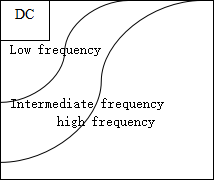
\includegraphics[width=0.3\textwidth]{Figure/2.png}
    \caption{Discrete Cosine Transform band distribution}
    \label{fig:2-2}
\end{figure}

\section{Walsh Transform}

The transformation matrix of the Walsh Transform is simple, only 1 and -1, which takes up less storage space, is easy to generate, has a fast algorithm, is widely used in image processing problems for processing large amounts of data in real time[9]. The Walsh Transform only needs to perform real-number operations, the stroage capacity is much less than the Fast Fourier Transfrom, so the operation speed is much faster. It is better than Fast Fourier Transform to use it to approximate the digital pulse signal data. The Walsh Transform has the characteristics of energy concentration, the more uniform the data distribution in the original data, the more data is concentrated on the corners of the matrix. Therefore, Walsh Transform is widely used in the fields of image transmission, telecommunication technology, and data compression.and so on.

%添加表格的方法
\begin{table}[htbp]
    \centering
    \caption{Your table caption}
    \label{tab:2-1}
    \begin{tabular}{ccc} %三列表格，全部居中
        \toprule % 顶部横线
        Header 1 & Header 2 & Header 3 \\
        \midrule % 中部横线
        Data 1 & Data 2 & Data 3 \\
        Data 4 & Data 5 & Data 6 \\
        \bottomrule % 底部横线
    \end{tabular}
\end{table}

%添加空白页，根据需要灵活取舍
\clearpage
\null
\clearpage